\documentclass[10pt,mathserif]{beamer}

% ------------------------------------------------------------------------
% Packages
% ------------------------------------------------------------------------
\usepackage{amsmath}
\usepackage{tabularx}

% ------------------------------------------------------------------------
% Macros
% ------------------------------------------------------------------------
%~~~~~~~~~~~~~~~
% List shorthand
%~~~~~~~~~~~~~~~
\newcommand{\BIT}{\begin{itemize}}
\newcommand{\EIT}{\end{itemize}}
\newcommand{\BNUM}{\begin{enumerate}}
\newcommand{\ENUM}{\end{enumerate}}
%~~~~~~~~~~~~~~~
% Text with quads around it
%~~~~~~~~~~~~~~~
\newcommand{\qtext}[1]{\quad\text{#1}\quad}
%~~~~~~~~~~~~~~~
% Shorthand for math formatting
%~~~~~~~~~~~~~~~
\newcommand\mbb[1]{\mathbb{#1}}
\newcommand\mbf[1]{\mathbf{#1}}
\def\mc#1{\mathcal{#1}}
\def\mrm#1{\mathrm{#1}}
%~~~~~~~~~~~~~~~
% Common sets
%~~~~~~~~~~~~~~~
\def\reals{\mathbb{R}} % Real number symbol
\def\integers{\mathbb{Z}} % Integer symbol
\def\rationals{\mathbb{Q}} % Rational numbers
\def\naturals{\mathbb{N}} % Natural numbers
\def\complex{\mathbb{C}} % Complex numbers
\def\simplex{\mathcal{S}} % Simplex
%~~~~~~~~~~~~~~~
% Common functions
%~~~~~~~~~~~~~~~
\renewcommand{\exp}[1]{\operatorname{exp}\left(#1\right)} % Exponential
\def\indic#1{\mbb{I}\left({#1}\right)} % Indicator function
\providecommand{\maximize}{\mathop\mathrm{maximize}} % Defining math symbols
\providecommand{\minimize}{\mathop\mathrm{minimize}}
\providecommand{\argmax}{\mathop\mathrm{arg max}}
\providecommand{\argmin}{\mathop\mathrm{arg min}}
\providecommand{\arccos}{\mathop\mathrm{arccos}}
\providecommand{\asinh}{\mathop\mathrm{asinh}}
\providecommand{\dom}{\mathop\mathrm{dom}} % Domain
\providecommand{\range}{\mathop\mathrm{range}} % Range
\providecommand{\diag}{\mathop\mathrm{diag}}
\providecommand{\tr}{\mathop\mathrm{tr}}
\providecommand{\abs}{\mathop\mathrm{abs}}
\providecommand{\card}{\mathop\mathrm{card}}
\providecommand{\sign}{\mathop\mathrm{sign}}
\def\rank#1{\mathrm{rank}({#1})}
\def\supp#1{\mathrm{supp}({#1})}
%~~~~~~~~~~~~~~~
% Common probability symbols
%~~~~~~~~~~~~~~~
\def\E{\mathbb{E}} % Expectation symbol
\def\Earg#1{\E\left[{#1}\right]}
\def\Esubarg#1#2{\E_{#1}\left[{#2}\right]}
\def\P{\mathbb{P}} % Probability symbol
\def\Parg#1{\P\left({#1}\right)}
\def\Psubarg#1#2{\P_{#1}\left[{#2}\right]}
\def\Cov{\mrm{Cov}} % Covariance symbol
\def\Corr{\mrm{Corr}} % Covariance symbol
\def\Covarg#1{\Cov\left[{#1}\right]}
\def\Covsubarg#1#2{\Cov_{#1}\left[{#2}\right]}
\def\Corrsubarg#1#2{\Corr_{#1}\left[{#2}\right]}
\def\Var{\mrm{Var}}
\def\Vararg#1{\Var\left(#1\right)}
\def\Varsubarg#1#2{\Var_{#1}\left(#2\right)}
\newcommand{\family}{\mathcal{P}} % probability family
\newcommand{\eps}{\epsilon}
\def\absarg#1{\left|#1\right|}
\def\msarg#1{\left(#1\right)^{2}}
\def\logarg#1{\log\left(#1\right)}
%~~~~~~~~~~~~~~~
% Distributions
%~~~~~~~~~~~~~~~
\def\Gsn{\mathcal{N}}
\def\Ber{\textnormal{Ber}}
\def\Bin{\textnormal{Bin}}
\def\Unif{\textnormal{Unif}}
\def\Mult{\textnormal{Mult}}
\def\Cat{\textnormal{Cat}}
\def\Gam{\textnormal{Gam}}
\def\InvGam{\textnormal{InvGam}}
\def\NegMult{\textnormal{NegMult}}
\def\Dir{\textnormal{Dir}}
\def\Lap{\textnormal{Laplace}}
\def\Bet{\textnormal{Beta}}
\def\Poi{\textnormal{Poi}}
\def\HypGeo{\textnormal{HypGeo}}
\def\GEM{\textnormal{GEM}}
\def\BP{\textnormal{BP}}
\def\DP{\textnormal{DP}}
\def\BeP{\textnormal{BeP}}
%~~~~~~~~~~~~~~~
% Theorem-like environments
%~~~~~~~~~~~~~~~

%-----------------------
% Probability sets
%-----------------------
\newcommand{\X}{\mathcal{X}}
\newcommand{\Y}{\mathcal{Y}}
\newcommand{\D}{\mathcal{D}}
\newcommand{\Scal}{\mathcal{S}}
%-----------------------
% vector notation
%-----------------------
\newcommand{\bx}{\mathbf{x}}
\newcommand{\by}{\mathbf{y}}
\newcommand{\bt}{\mathbf{t}}
\newcommand{\xbar}{\overline{x}}
\newcommand{\Xbar}{\overline{X}}
\newcommand{\tolaw}{\xrightarrow{\mathcal{L}}}
\newcommand{\toprob}{\xrightarrow{\mathbb{P}}}
\newcommand{\laweq}{\overset{\mathcal{L}}{=}}
\newcommand{\F}{\mathcal{F}}

\usepackage{graphicx,amsmath,amssymb,natbib}

%% formatting
\setbeamertemplate{navigation symbols}{}
\usecolortheme[rgb={0.13,0.28,0.59}]{structure}
\setbeamertemplate{itemize subitem}{--}
\setbeamertemplate{frametitle} {
	\begin{center}
	  {\large\bf \insertframetitle}
	\end{center}
}

\newcommand\footlineon{
  \setbeamertemplate{footline} {
    \begin{beamercolorbox}[ht=2.5ex,dp=1.125ex,leftskip=.8cm,rightskip=.6cm]{structure}
      \footnotesize \insertsection
      \hfill
      {\insertframenumber}
    \end{beamercolorbox}
    \vskip 0.45cm
  }\begin{figure}[ht]
  \centering
\end{figure}

}
%% begin presentation

\title{\large \bfseries Generative Adversarial Networks}

\author{Kris Sankaran\\[3ex]
Nepal Winter School in AI}

\date{\today}

\begin{document}

\frame{
  \thispagestyle{empty}
  \titlepage
}

\section{Introduction}

\begin{frame}
  \frametitle{Learning Objectives}
 \begin{itemize}
  \item Understand basic adversarial setup
  \item Mathematical perspectives to help navigate sea of proposed variants
  \item Get a flavor of some real-world applications
 \end{itemize}
\end{frame}

\begin{frame}
  \frametitle{First thing that comes to mind?}
\begin{itemize}
\item GANs are popular ways to generate images
\end{itemize}
\begin{figure}[ht]
  \centering
  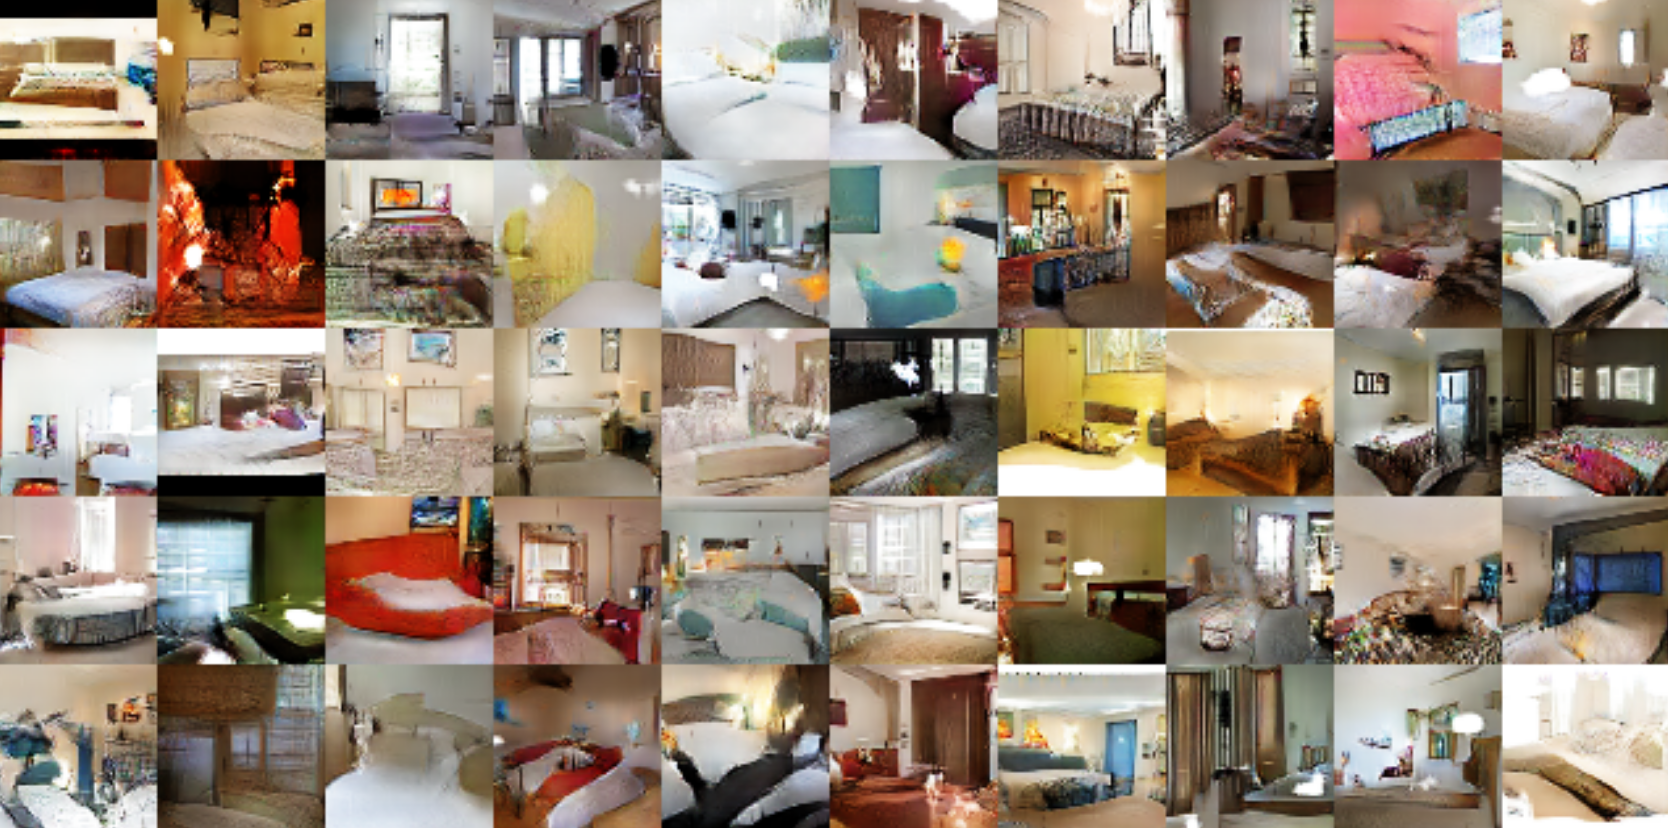
\includegraphics[width=0.7\paperwidth]{figure/gan_example}
  \caption{Probably the most famous GAN samples of all
    time. \citep{radford2015unsupervised} \label{fig:gan_example} }
\end{figure}
\end{frame}

\begin{frame}
  \frametitle{Or maybe this?}
\begin{itemize}
\item GANs are popular ways to generate images
\end{itemize}
\begin{figure}[ht]
  \centering
  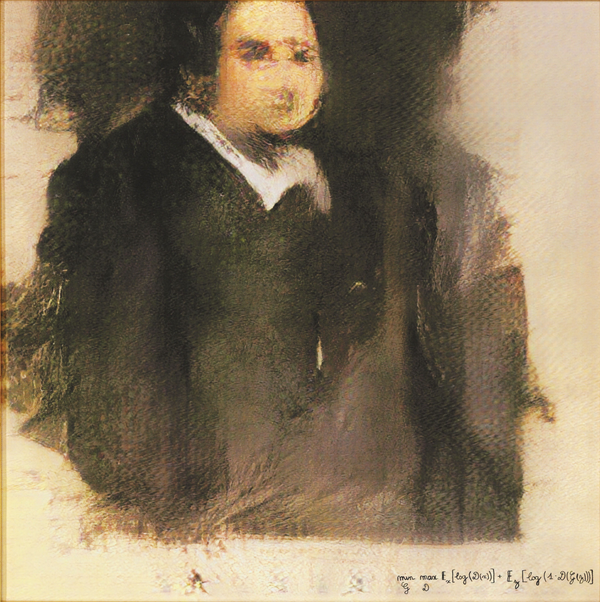
\includegraphics[width=0.3\paperwidth]{figure/gan_portrait.jpg}
  \caption{Probably the most expensive GAN sample of all
    time. \label{fig:gan_portrait} }
\end{figure}
\end{frame}

\begin{frame}
  \frametitle{GANs as Sampling Algorithms}
  \begin{itemize}
  \item Ignore the hype
  \item It's better to think of GANs as learning how to sample from probability
    densities $p\left(x\right)$
    \begin{itemize}
    \item For $32 \times 32$ images, $p\left(x\right)$ is a distribution in
      1024-dimensional space
    \end{itemize}
  \item What's exciting is that they are \textit{implicit} probability models
    \begin{itemize}
    \item Distribution defined implicitly by sampling mechanism
    \end{itemize} 
  \end{itemize}
  \begin{figure}[ht]
    \centering
    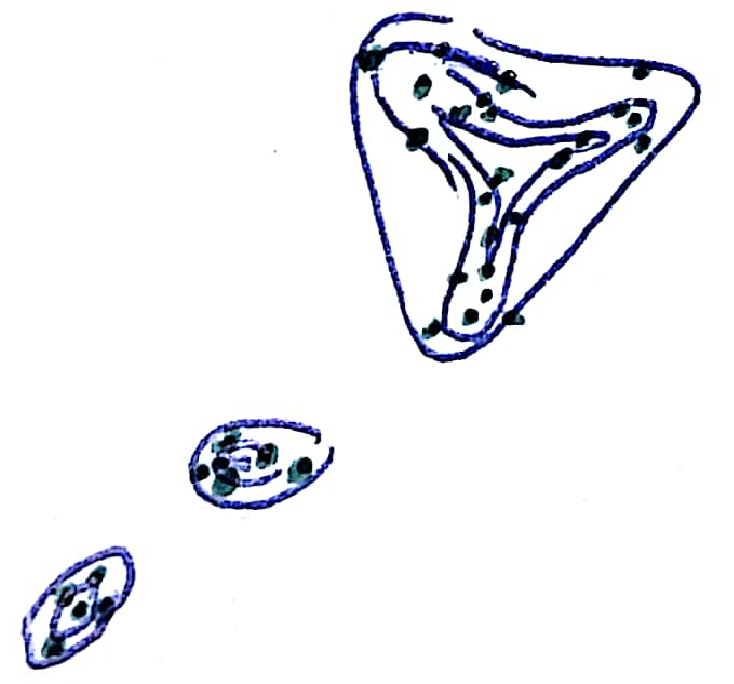
\includegraphics[width=0.3\paperwidth]{figure/gan_density}
    \caption{We may not be able to write simple formulas for complicated
      densities, but we may be able to write computer programs that sample from
      them.\label{fig:gan_density} }
  \end{figure}
\end{frame}

\begin{frame}
  \frametitle{Images and Probability}
\begin{itemize}
\item It's common in the GANs literature to show interpolations between
  generated images
\end{itemize}
\begin{figure}[ht]
  \centering
  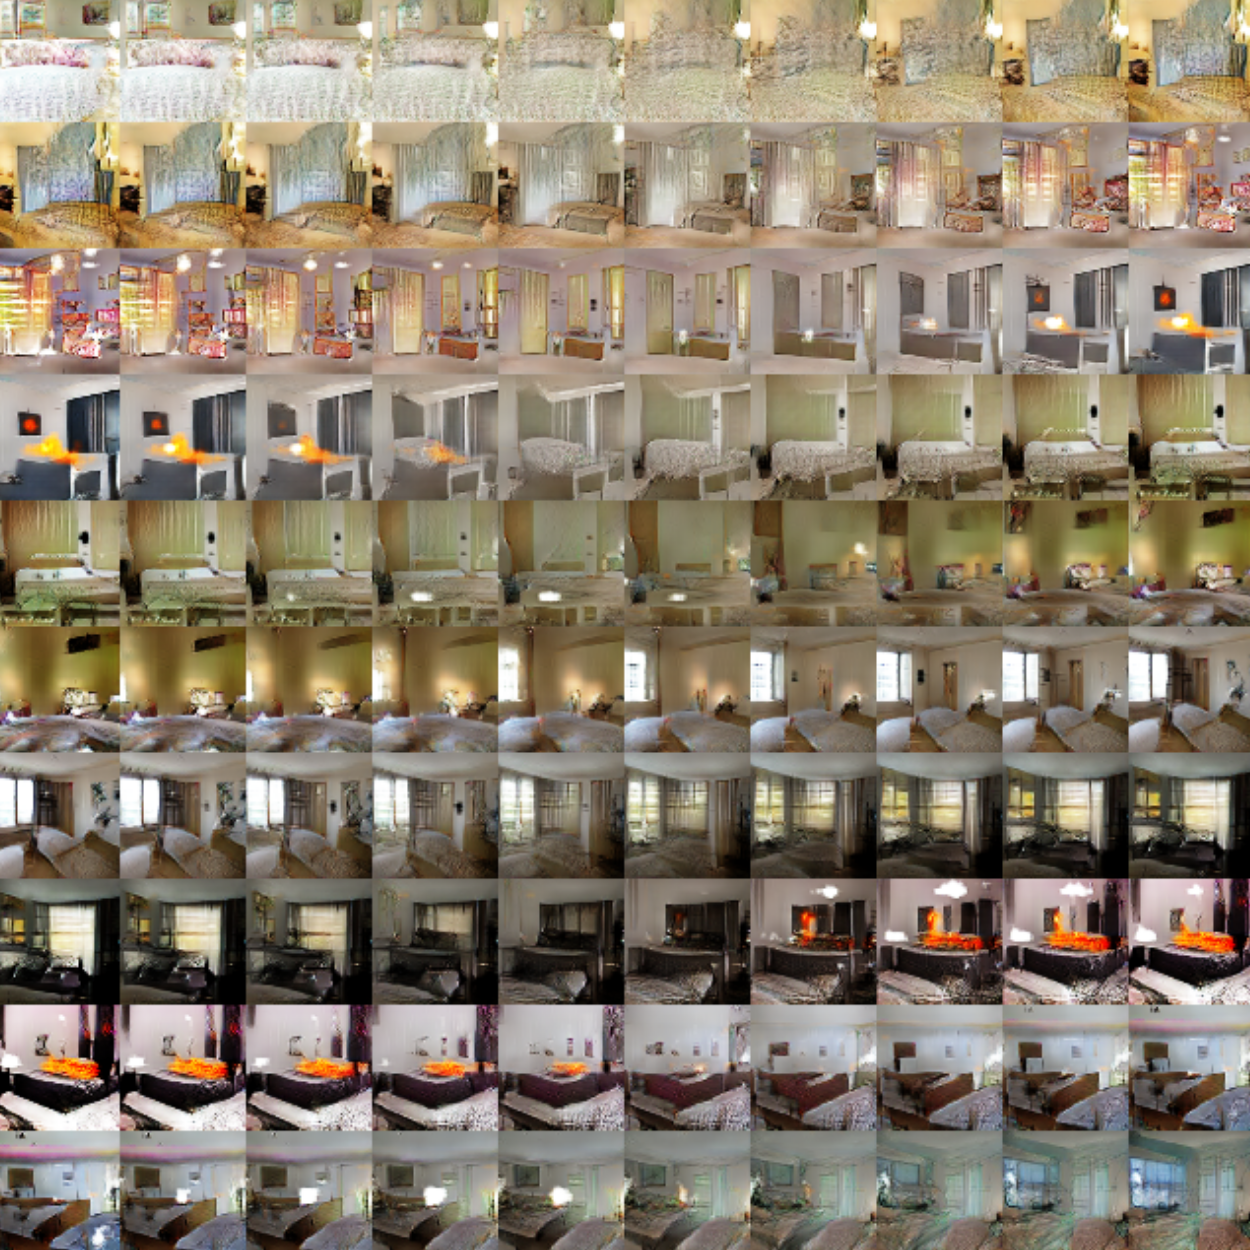
\includegraphics[width=0.35\paperwidth]{figure/gan_image_interpolations}
  \caption{Example interpolations between LSUN images in
    \citep{radford2015unsupervised}. This was a convincing result at the time,
    because it showed that the samples weren't simply memorized training
    data. \label{fig:gan_interpolations} }
\end{figure}
\end{frame}

\begin{frame}
  \frametitle{Images and Probability}
\begin{itemize}
  \item Geometrically, these interpolated images are points along a curve in
    image space
\end{itemize}
\begin{figure}[ht]
  \centering
  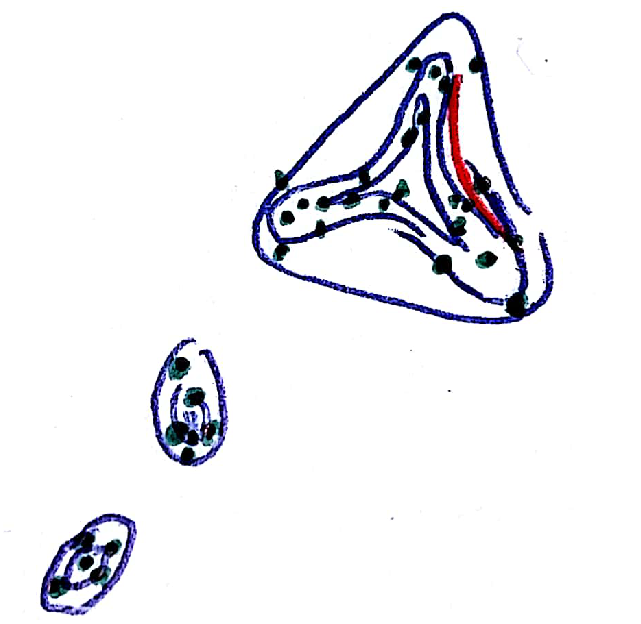
\includegraphics[width=0.3\paperwidth]{figure/gan_interpolations}
  \caption{The green points would each be an image, and the red line represents
    a sequence of gradually evolving samples, which should look like real
    images, if they live in a region of high probability.
    \label{fig:gan_interpolations_density} }
\end{figure}
\end{frame}

\section{Formulation}

\begin{frame}
  \frametitle{Formulation}
 \begin{itemize}
 \item How to transform (say, uniform) noise $z$ into arbitrary distributions?
 \item Idea: Use a neural network $G$
 \item $z \rightarrow G\left(z\right)$
 \end{itemize}
\begin{figure}[ht]
  \centering
  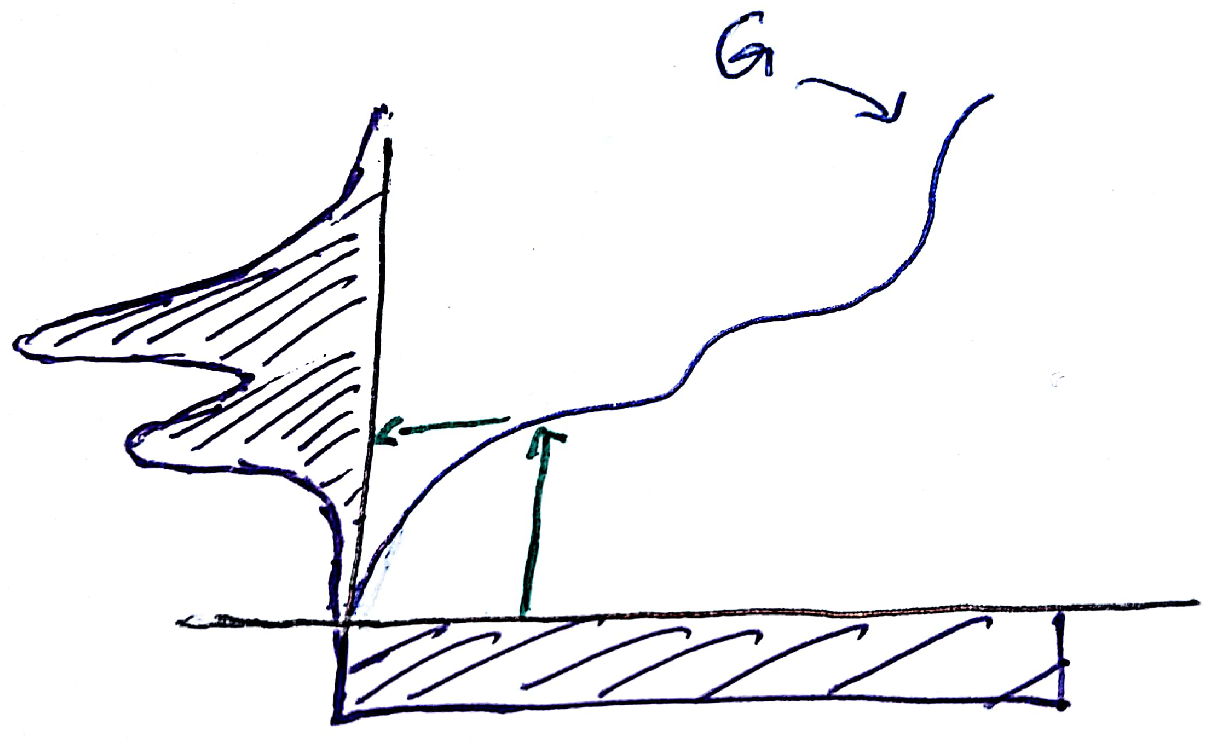
\includegraphics[width=0.52\paperwidth]{figure/sample_transformation}
  \caption{By passing samples from a probability distribution through a
    function, you get another probability distribution. $y$-values where the
    function is flatter will get more of the original mass, resulting in peaks
    in the transformed distribution. \label{fig:sample_transformation} }
\end{figure}
\end{frame}

\begin{frame}
  \frametitle{Formulation}
 \begin{itemize}
 \item How to learn a transformation to match observed data?
 \item Idea: Use another neural network! Call it $D$.
 \item This is pretty different from usual likelihood-based views
   \begin{itemize}
   \item (there are connections though)
   \end{itemize}
 \end{itemize}
\begin{figure}[ht]
  \centering
  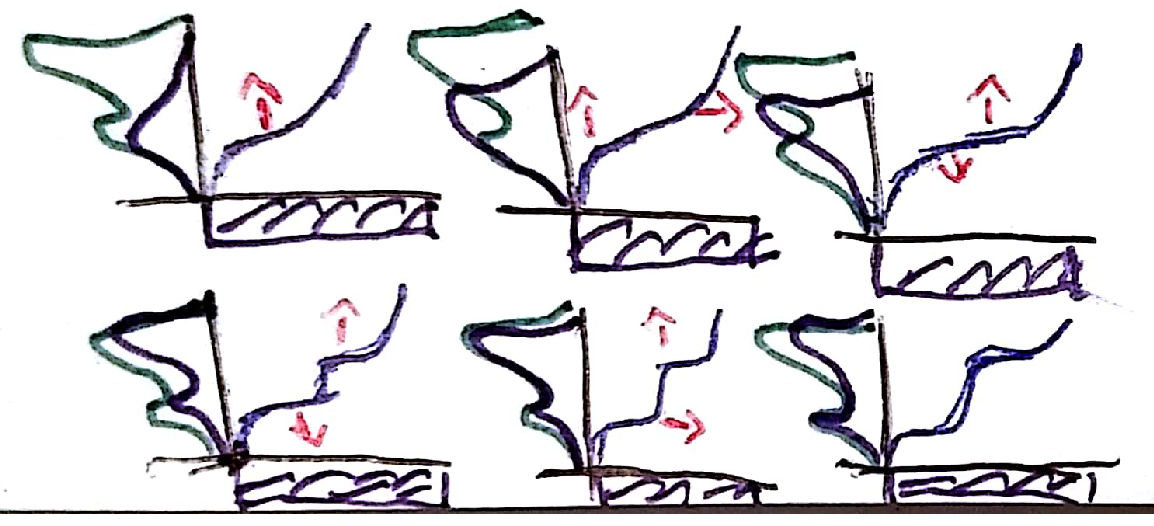
\includegraphics[width=0.7\paperwidth]{figure/discriminator_transformation}
  \caption{The discriminator guides the generator towards learning a good
    transformation, attempting to tell the difference between the true data
    (green) and generated (blue)
    distributions. \label{fig:discriminator_transformation} }
\end{figure}
\end{frame}

\begin{frame}
\frametitle{Objective Function}
 \begin{itemize}
   \item How should $D$ guide updates to $G$?
   \item Objective function
     \begin{align*}
       \min_{G}\max_{D} V\left(D, G\right) = \Esubarg{p_{\text{data}}}{D\left(x\right)} + \Esubarg{p\left(z\right)}{\log\left(1 - D\left(G\left(z\right)\right)\right)}
     \end{align*}
   \item Alternate gradient steps, first update $D$, then $G$, then $D$, ...
\begin{itemize}
\item $D$ tries to be large on $x$ and small on $G\left(z\right)$
\item $G$ is encouraged to make $D$ assign values near 1 to samples
  $G\left(z\right)$, so that the objective gets small
\end{itemize}
 \end{itemize}
\begin{figure}[ht]
  \centering
  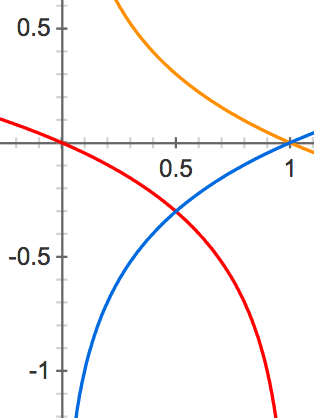
\includegraphics[width=0.17\paperwidth]{figure/gan_objectives}
  \caption{The blue, red, and orange lines are $\log x$, $\log\left(1 -
    x\right)$ and $-\log x$, respectively. This last function is often used
    instead of $\log \left(1 - x\right)$. \label{fig:gan_objectives} }
\end{figure}
\end{frame}

\begin{frame}
  \frametitle{GAN Lab}
  \url{https://poloclub.github.io/ganlab/}
  \begin{figure}[ht]
    \centering
    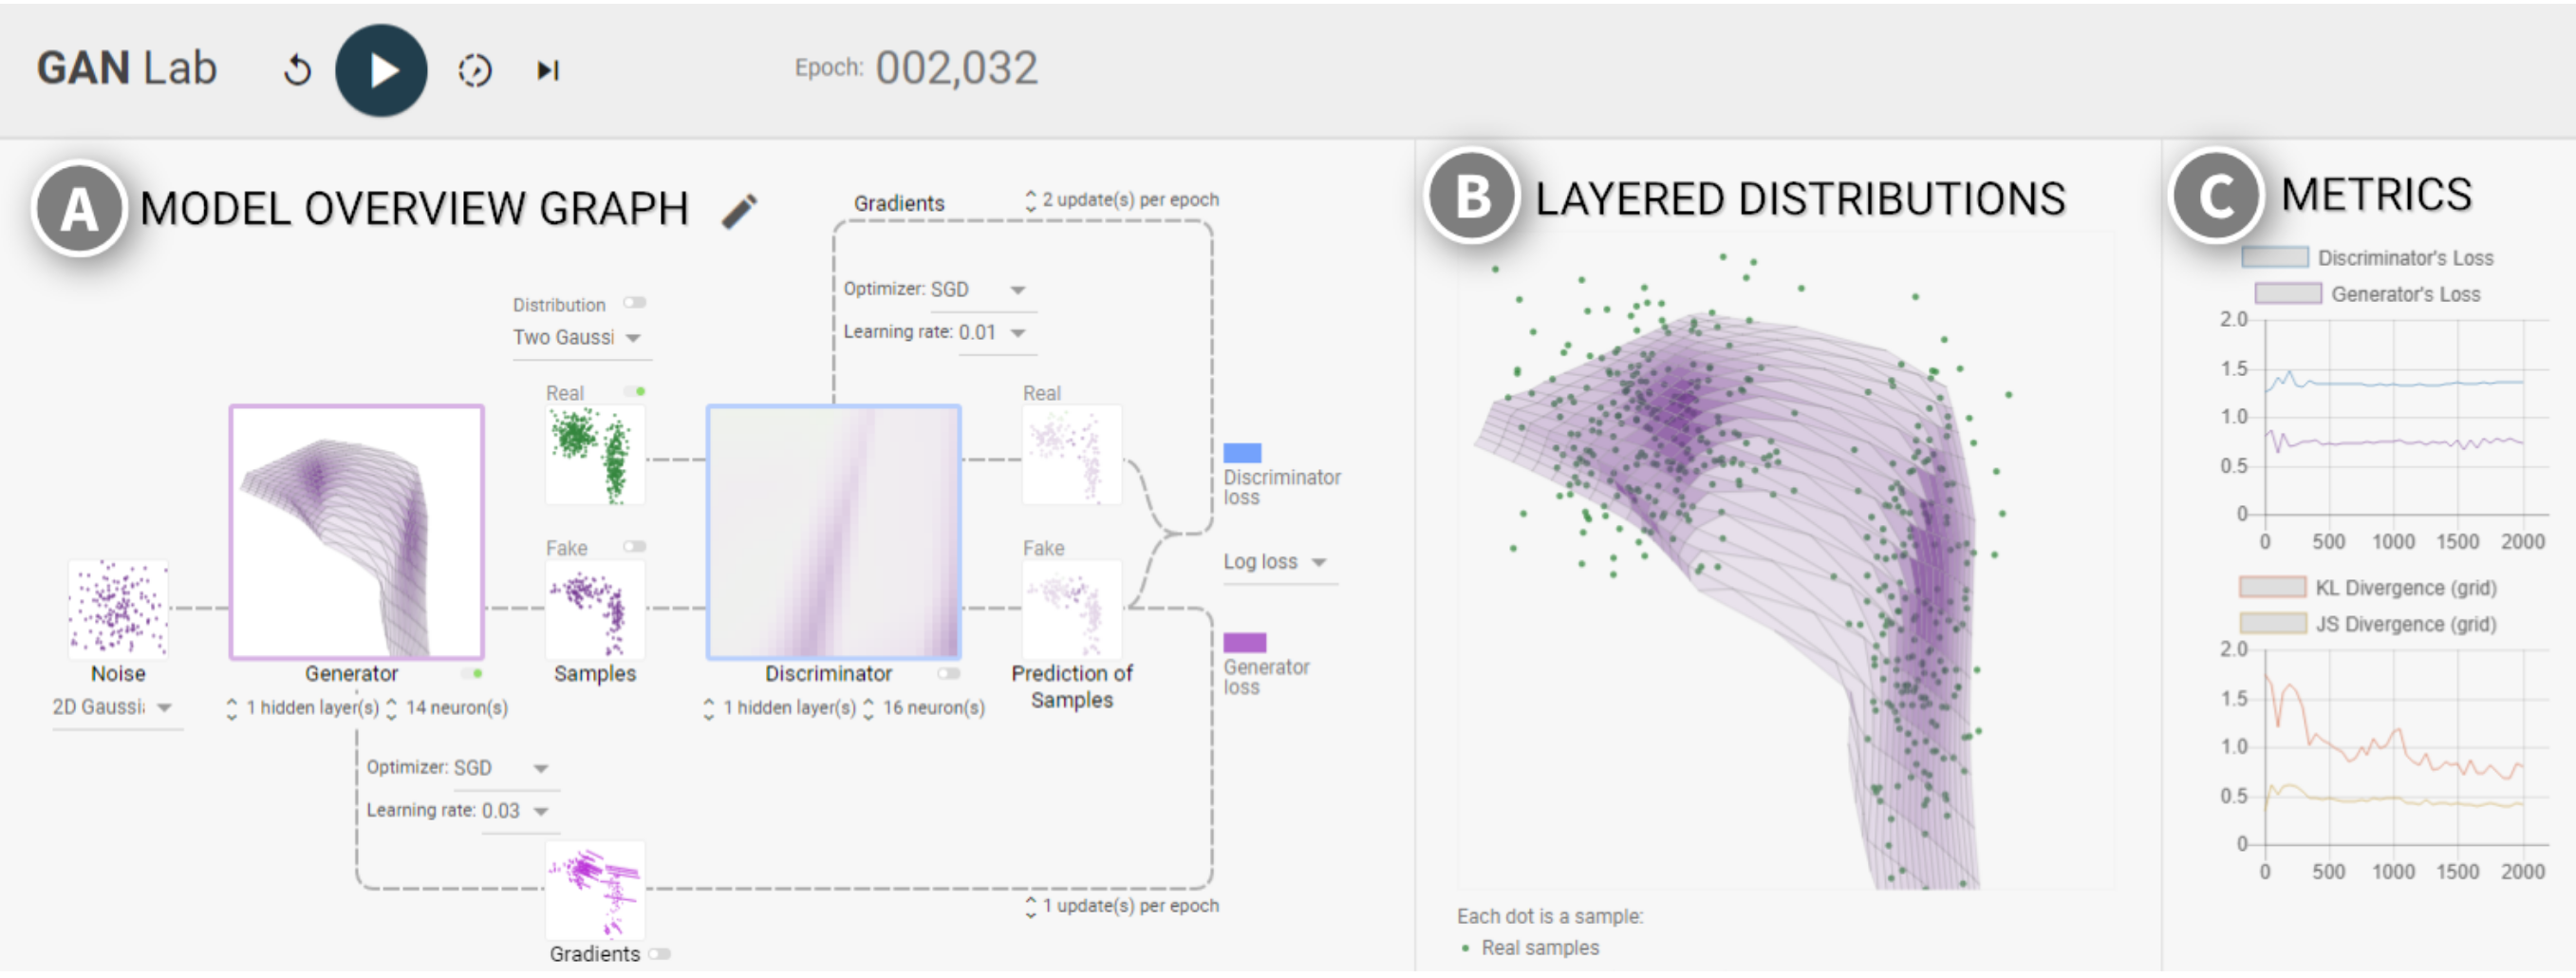
\includegraphics[width=0.7\paperwidth]{figure/ganlab}
    \caption{A visualization of the whole process, on a few different toy
      datasets. \label{fig:ganlab} }
  \end{figure}
\end{frame}

\section{Perspectives}
\label{sec:perspectives}

\begin{frame}
  \frametitle{Training difficulties}
 \begin{itemize}
 \item GANs have a bad reputation for being finnicky to train
 \item If the discriminator $D$ is ``too strong,'' it might not communicate
   useful information
 \end{itemize}
\begin{figure}[ht]
  \centering
  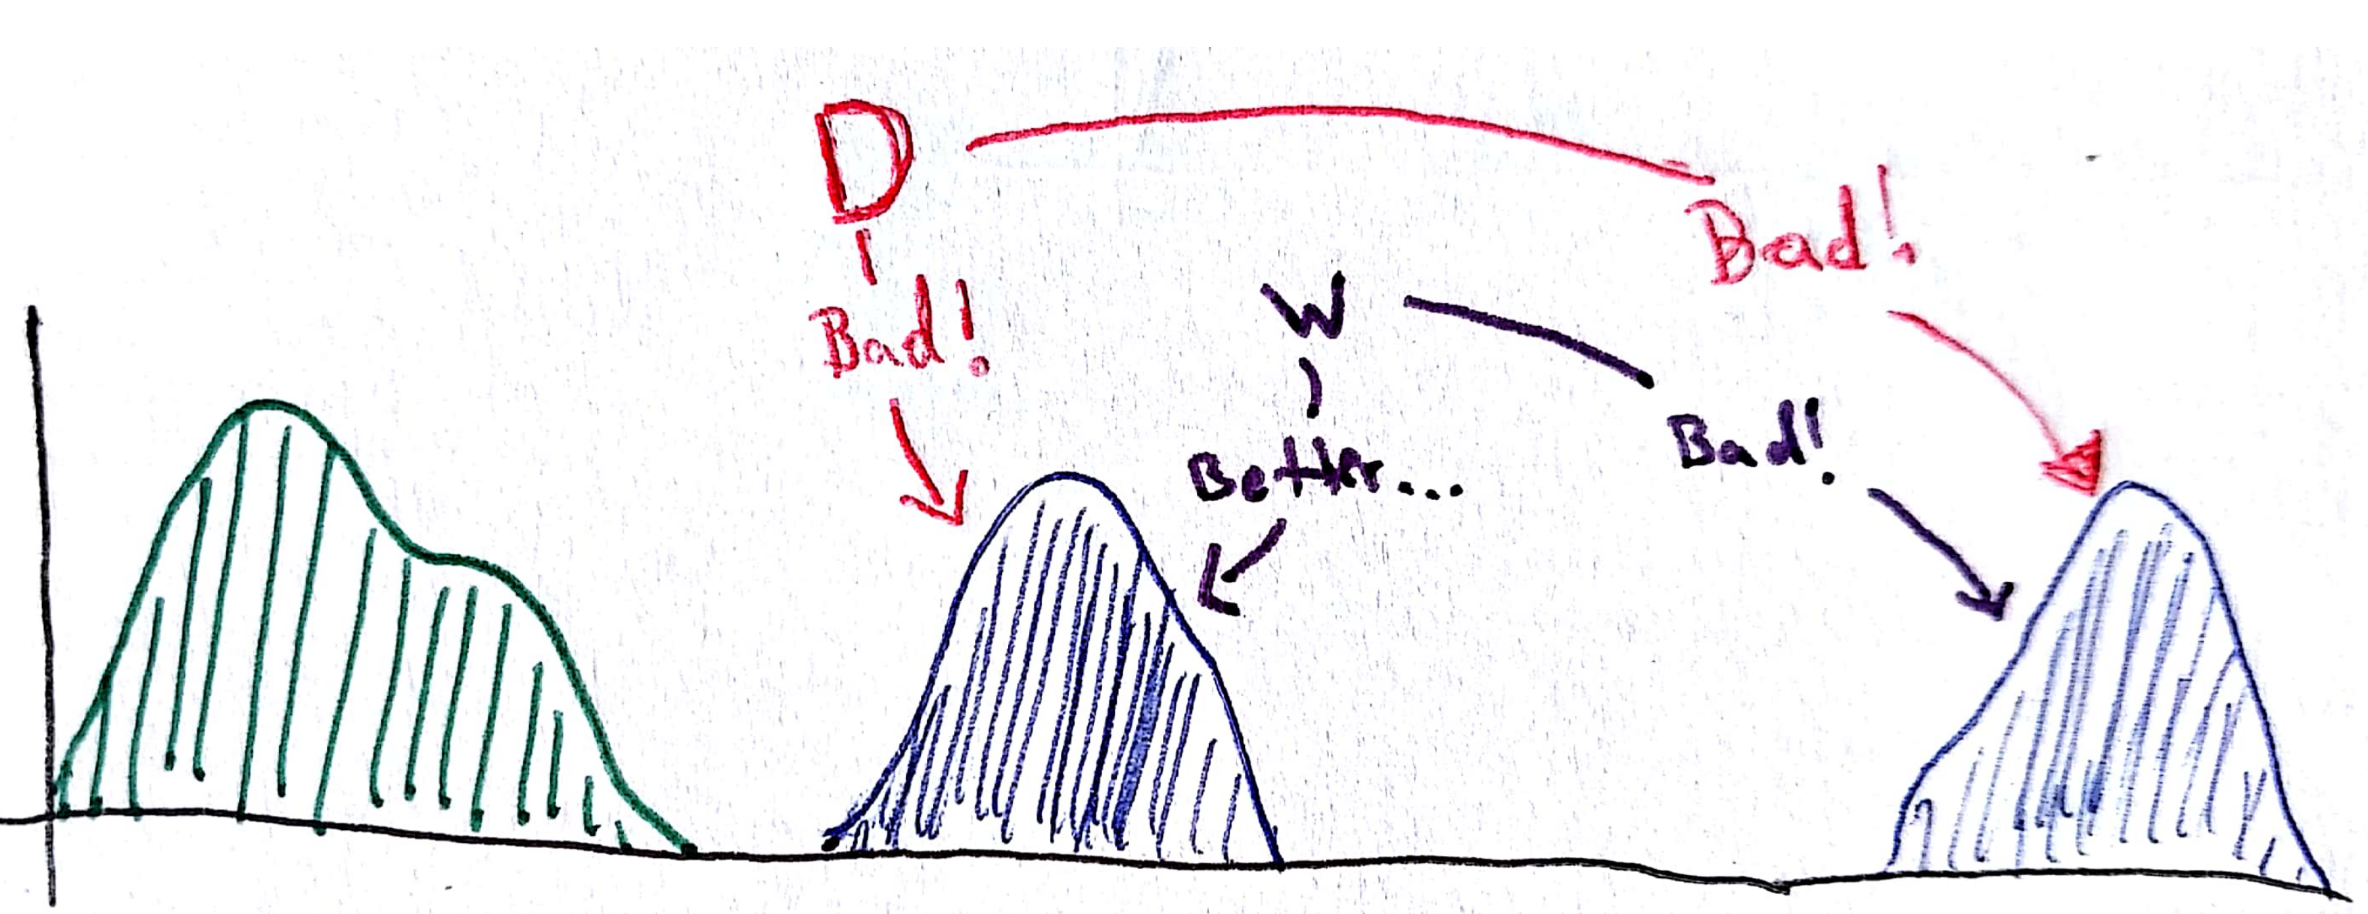
\includegraphics[width=0.7\paperwidth]{figure/alternative_critic}
  \caption{We would like a critic $W$ that tells the generator when it's getting
    closer, even when it's obviously different from the
    target. \label{fig:alternative_critic} }
\end{figure}
\end{frame}

\begin{frame}
  \frametitle{Wasserstein Distance}
 \begin{itemize}
 \item Formalize this idea using distances $d\left(\P_1, \P_2\right)$ between
   probability distributions
 \item KL-divergence compares densities \textit{vertically}
 \item Wasserstein compares densities \textit{horizontally}
 \item Wasserstein distance tells us something even when they are far away!
\end{itemize}
\begin{figure}[ht]
  \centering
  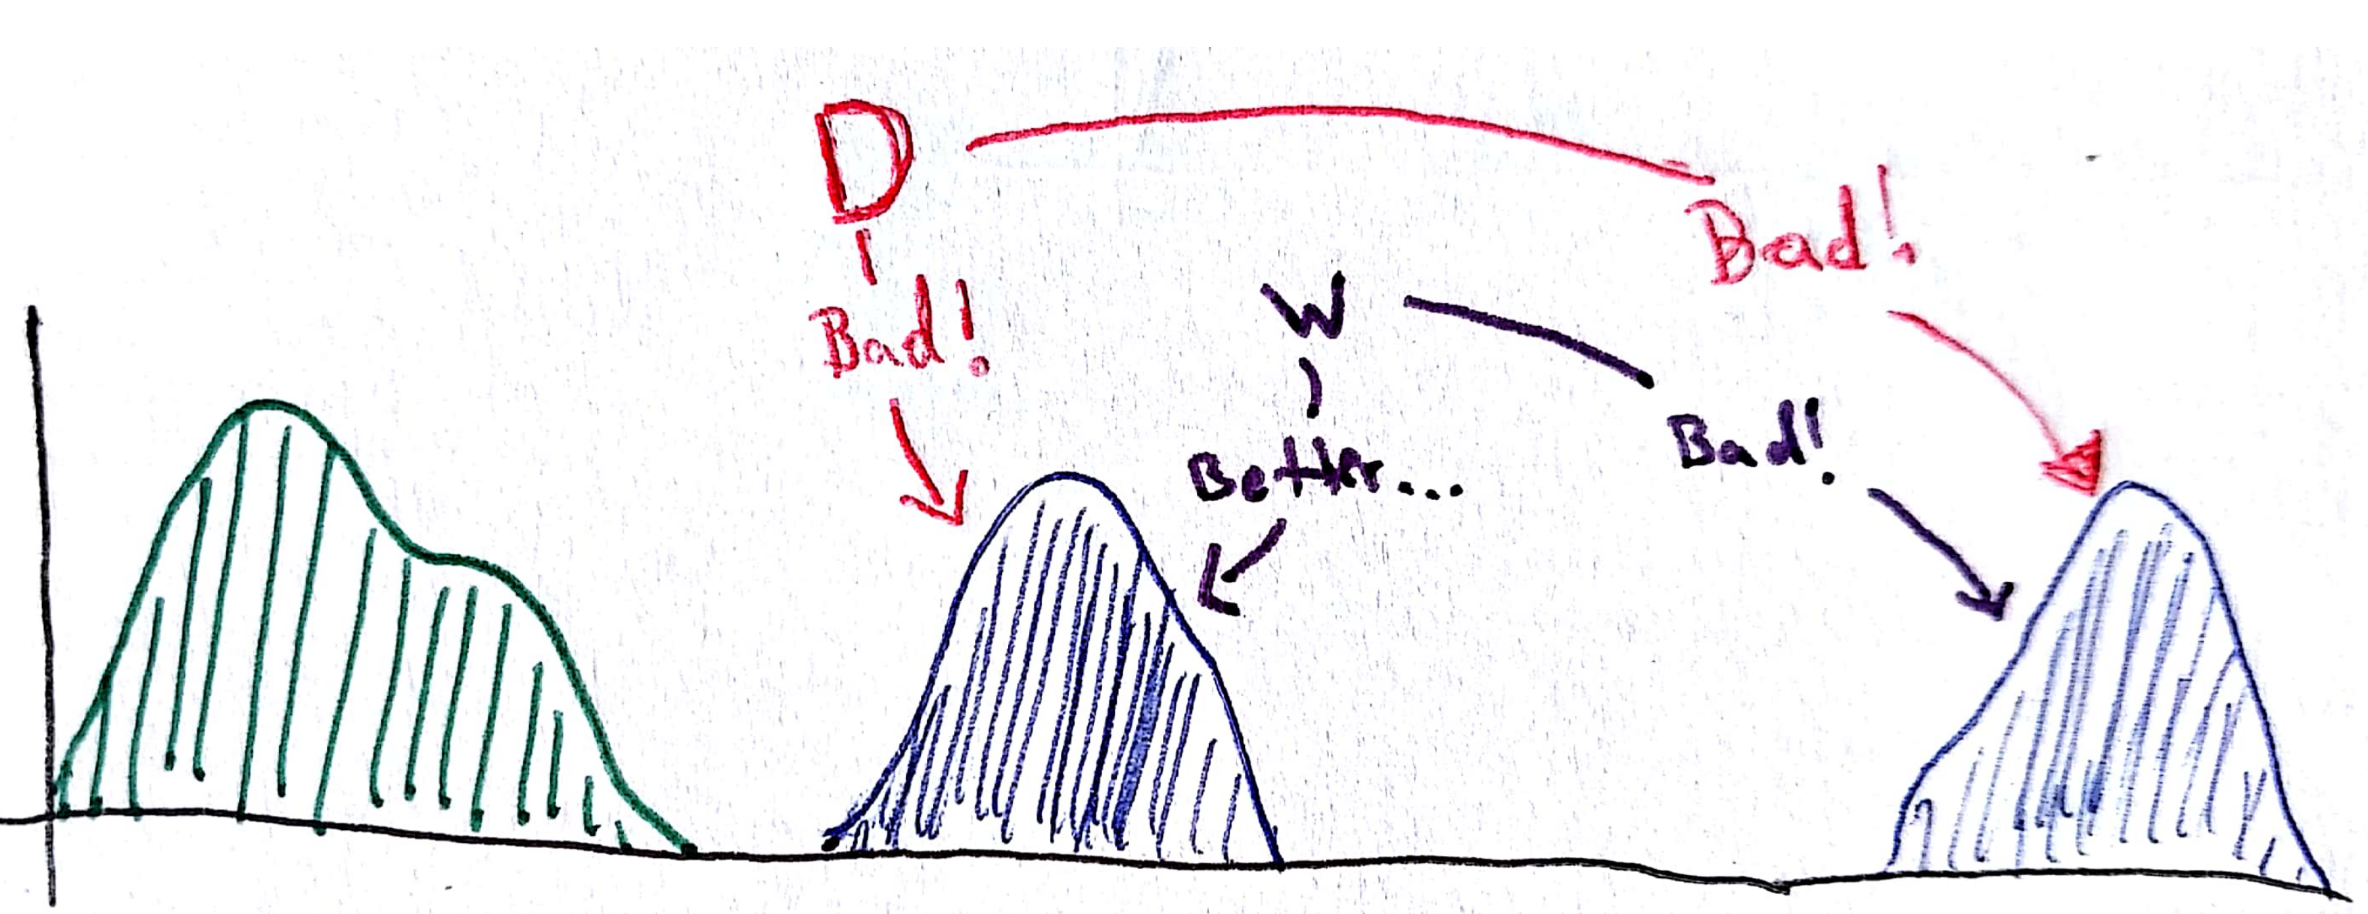
\includegraphics[width=0.7\paperwidth]{figure/alternative_critic}
  \caption{We would like a critic $W$ that tells the generator when it's getting
    closer, even when it's obviously different from the
    target. \label{fig:alternative_critic} }
\end{figure}
\end{frame}

\begin{frame}
  \frametitle{Wasserstein Objective}
  Wasserstein distance between data $X$ and generated $\tilde{X}$
  distributions is defined by
  \begin{align*}
    d\left(\P_X, \P_{\tilde{X}}\right) &= \max_{\|f\|_{L} \leq 1} \Esubarg{X}{f\left(x\right)} - \Esubarg{\tilde{X}}{f\left(\tilde{x}\right)}
  \end{align*}
  where $\|f\|_{L} \leq 1$ is the set of functions whose slopes are always less
  than 1.
  \begin{figure}[ht]
    \centering
    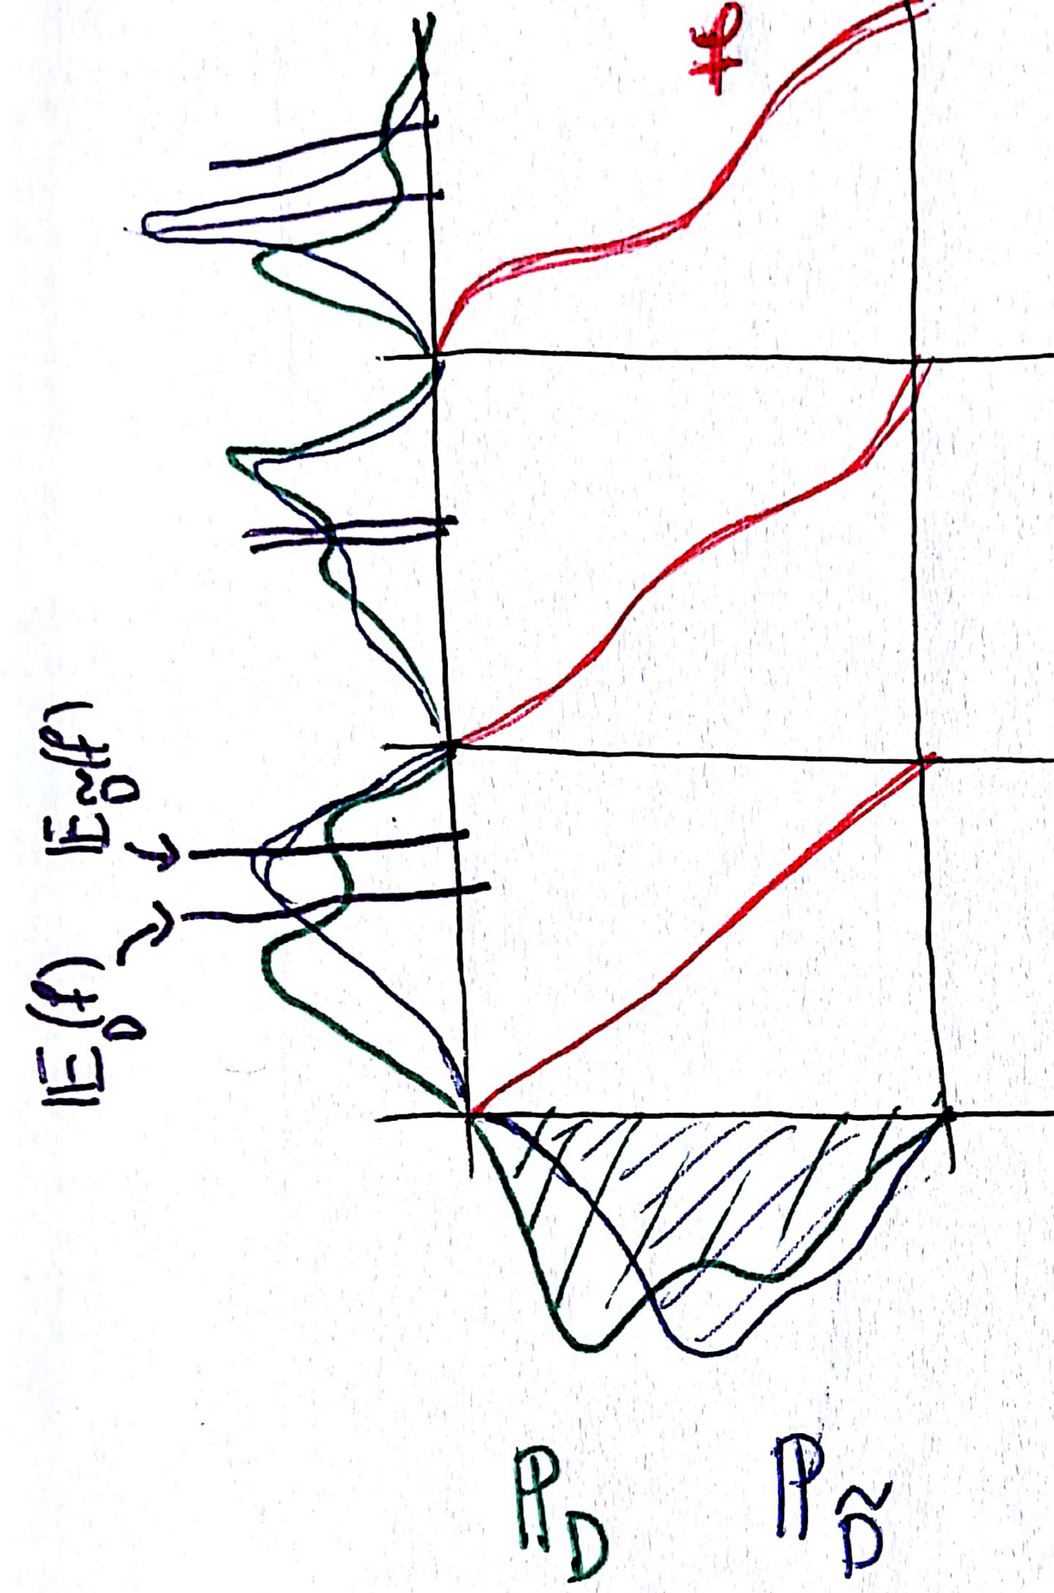
\includegraphics[width=0.2\paperwidth]{figure/wasserstein_tests}
    \caption{You can interpret the objective as computing differences in means
      after passing samples through a variety of (not too wild) test
      functions.\label{fig:wasserstein_tests} }
  \end{figure}
\end{frame}

\begin{frame}
  \frametitle{Wasserstein Training}
  \begin{itemize}
  \item In terms of the transformed noise $G\left(z\right)$, this looks like
    \begin{align*}
      d\left(\P_{X}, \P_{\tilde{X}}\right) &= \max_{\|f\| \leq 1} \Esubarg{X}{f\left(x\right)} - \Esubarg{Z}{f\left(G\left(z\right)\right)}
    \end{align*}
  \item Finding the optimal $f$ for any particular choice of $G$ is complicated...
  \item As an alternative, do gradient updates
  \begin{itemize}
  \item Critic $f$ inches towards its maximizing value of $d\left(\P_{X},
    \P_{\tilde{X}}\right)$.
  \item Generator $G$ descends towards smaller wasserstein distances
  \item Constraint $\|f\|_{L} \leq 1$ maintained either by clipping or
    regularization
  \end{itemize}
\end{itemize}
\end{frame}

\begin{frame}
  \frametitle{Implicit Learning}
  \begin{itemize}
  \item Alternative perspective: GANs as likelihood-free inference / implicit
    learning
  \item Remember generative mechanism,
    \begin{align*}
      z &\sim q\left(z\right) \\
      x \vert z &:= G_{\theta}\left(z\right)
    \end{align*}
  \item Marginal density $q_{\theta}\left(x\right)$ of data generated by this
    process is not analytically available
  \end{itemize}
\end{frame}

\begin{frame}
  \frametitle{Estimating Density Ratios}
 \begin{itemize}
 \item Let $p^{\ast}\left(x\right)$ be the true data generating density
 \item Let $y$ be an indicator of true vs. simulated data
   \begin{itemize}
   \item $p\left(x \vert y = 1\right) = p^{\ast}\left(x\right)$
   \item $p\left(x \vert y = 0\right) = q_{\theta}\left(x\right)$
   \end{itemize}
 \item We can't evaluate either $p^\ast$ or $q_{\theta}$ directly, but by Bayes' rule,
   \begin{align*}
     \frac{p^{\ast}\left(x\right)}{q_{\theta}\left(x\right)} &= \frac{p\left(y = 1 \vert x\right)p\left(x\right)}{p\left(y = 1\right)} \frac{p\left(y = 0\right)}{p\left(y = 0 \vert x\right)p\left(x\right)} \\
     &= \frac{p\left(y = 1 \vert x\right)}{p\left(y = 0 \vert x\right)} \frac{1 - \pi}{\pi}
   \end{align*}
   where $\pi = p\left(y = 1\right)$.
   \item We just need a classifier $D_{\varphi}\left(x\right)$ to tell difference between
     truth and simulated
 \end{itemize}
\end{frame}

\begin{frame}
  \frametitle{Learning}
 \begin{itemize}
 \item Lots of options: just specify what you are trying to do (ratio matching,
   density difference) and how you are going to get there (cross-entropy,
   f-divergence, ...)
 \item For example, if you try estimating density ratios using Bernoulli loss,
   \begin{align*}
     &\Esubarg{p\left(x \vert y\right)p\left(y\right)}{y \log D_{\varphi}\left(x\right) + \left(1 - y\right)\log \left(1 - D_{\varphi}\left(x\right)\right)} \\
      = & \pi \Esubarg{p\left(x \vert y = 1\right)}{\log D_{\varphi}\left(x\right)} + \left(1 - \pi\right)\Esubarg{p\left(x \vert y = 0\right)}{\log \left(1 - D_{\varphi}\left(x\right)\right)} \\
     = & \pi \Esubarg{p^{\ast}\left(x\right)}{\log D_{\varphi}\left(x\right)} + \left(1 - \pi\right)\Esubarg{q_{\theta}\left(x\right)}{\log \left(1 - D_{\varphi}\left(x\right)\right)}
   \end{align*}
  which is exactly the usual loss for GANs, if we set $\pi = \frac{1}{2}$.
 \end{itemize}
\end{frame}

\section{Applications}
\label{sec:applications}

\begin{frame}
  \frametitle{Applications: Image-to-Image translation}
\begin{figure}[ht]
  \centering
  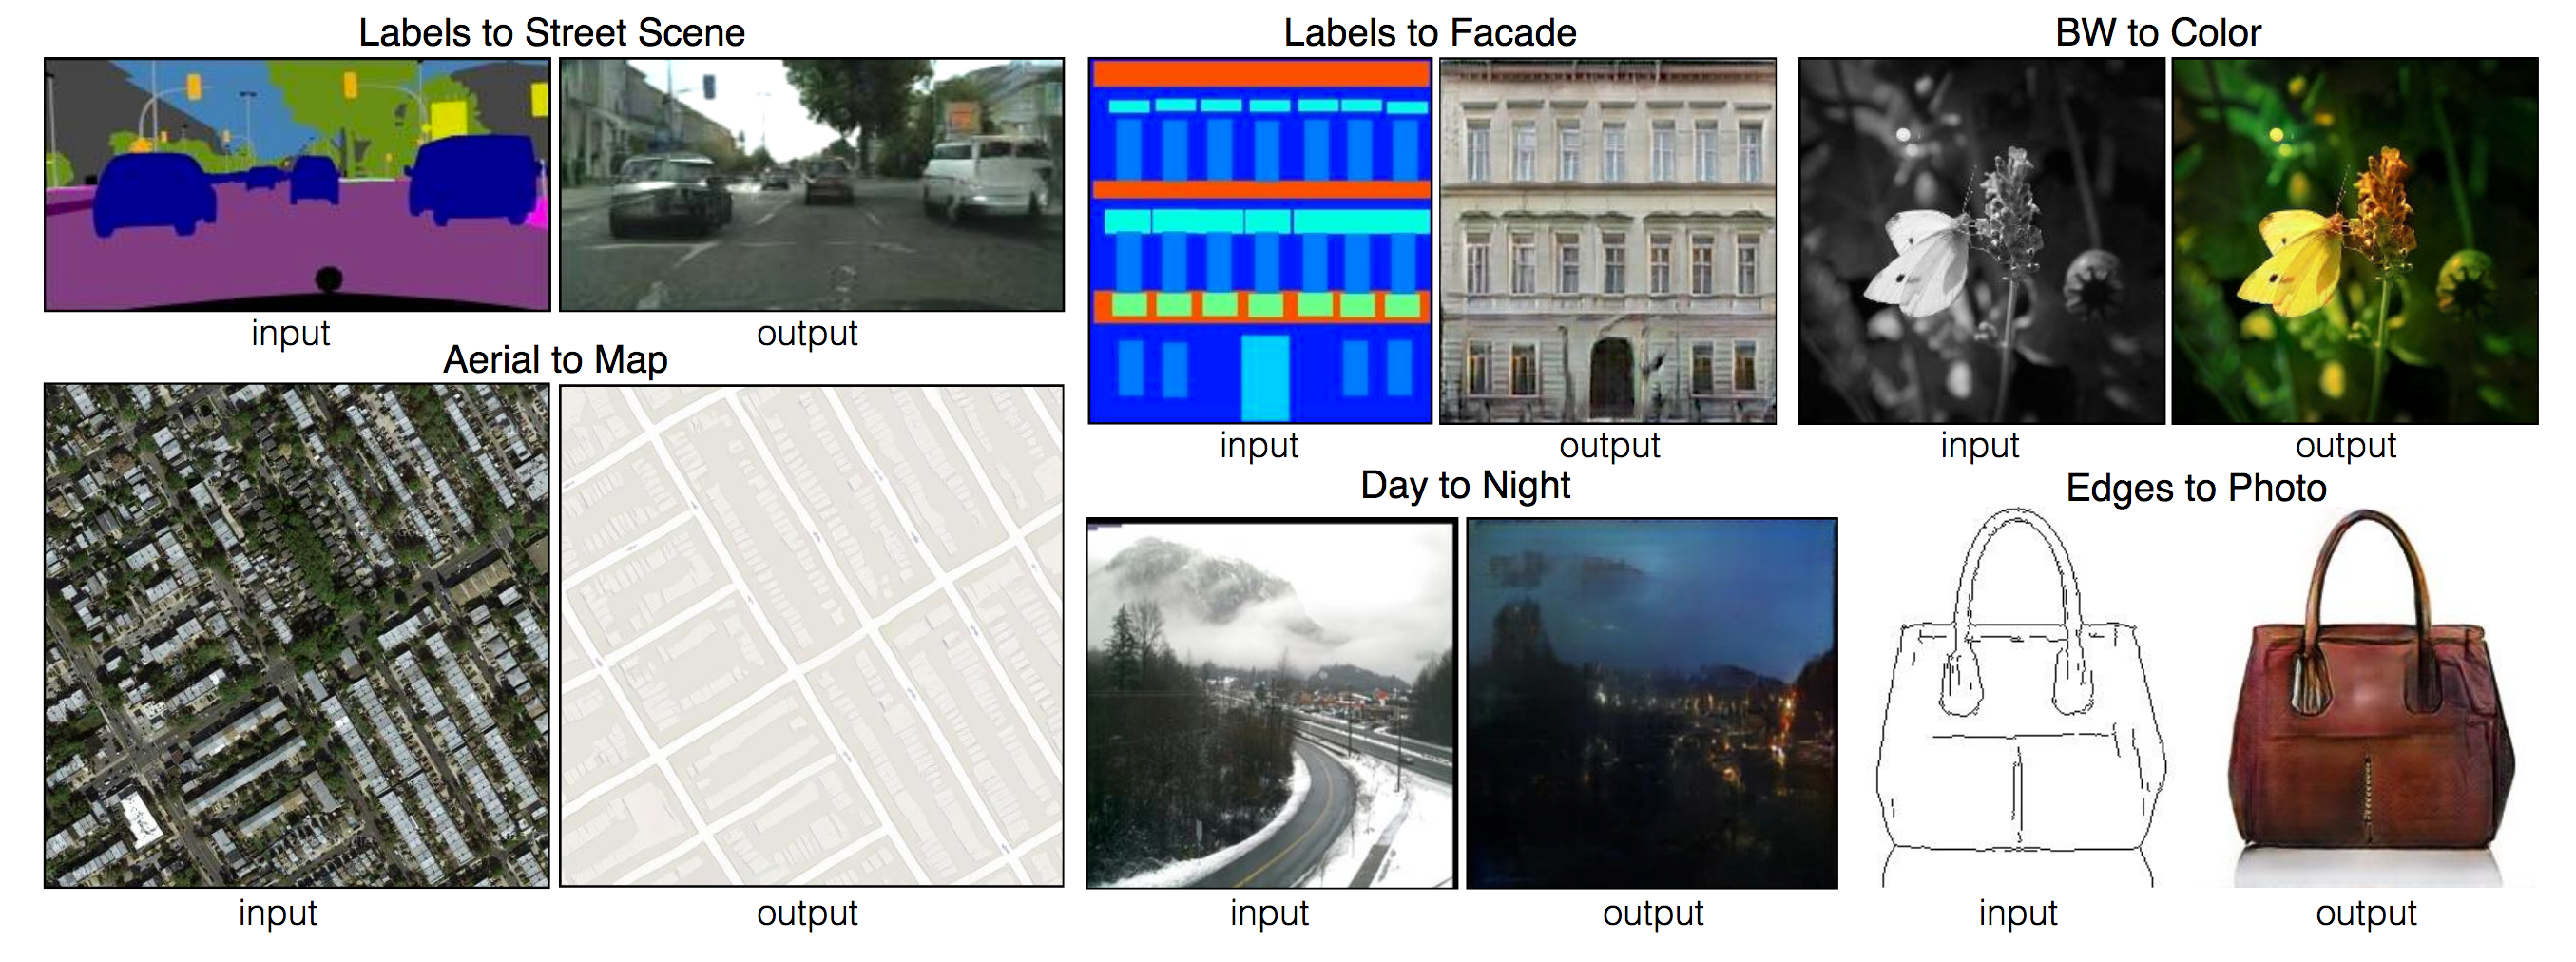
\includegraphics[width=0.9\paperwidth]{figure/image_to_image}
  \caption{Adding on a GAN objective when learning to map one class of images to
    another results in realistic looking translated
    images. \label{fig:image_to_image} }
\end{figure}
\end{frame}

\begin{frame}
  \frametitle{Applications: Inpainting}
\begin{figure}[ht]
  \centering
  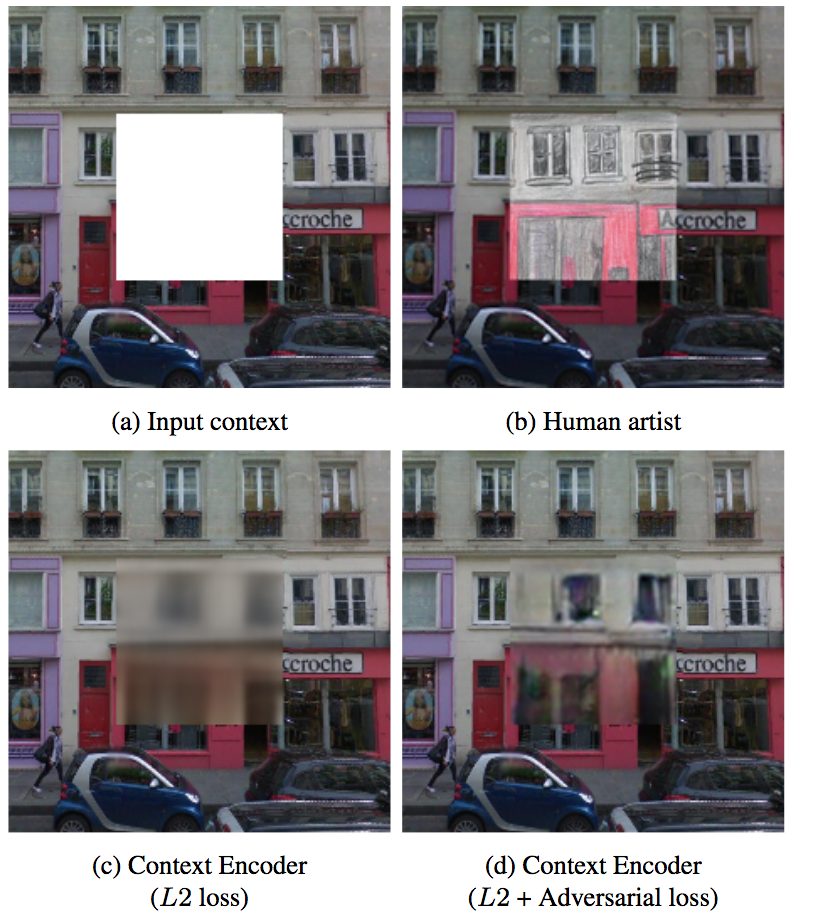
\includegraphics[width=0.45\paperwidth]{figure/inpainting}
  \caption{Similarly, when applied to inpainting, the GAN loss leads to much
    less blurry images than the traditional $\ell^{2}$
    loss. \label{fig:inpainting} }
\end{figure}
\end{frame}

\begin{frame}
  \frametitle{Applications: Super-Resolution}
  \begin{figure}[ht]
  \centering
  \includegraphics[width=0.9\paperwidth]{figure/srgan}
  \caption{It's interesting to note that some of the details that appear in the
    GAN super-resolved image were not present in the original high-resolution
    version.}
  \end{figure}
\end{frame}

\begin{frame}
  \frametitle{Conclusion}
  \begin{itemize}
    \item GANs are generic unsupervised learning procedure that don't require
      explicit probability densities
    \item They learn to transform simple distributions into those that resemble training data
    \item They can be used in many computer vision problems
  \end{itemize}
\end{frame}

\bibliography{refs}
\end{document}
